\documentclass[11pt,a4paper]{article}

\newcommand{\tumsoTime}{13:00 น. - 16:00 น.}
\newcommand{\tumsoRound}{2}

\usepackage{../tumso}

\begin{document}

\begin{problem}{Tetris Battle}{standard input}{standard output}{1 seconds}{256 megabytes}{100}

Tetris เกมต่อบล็อกขนาด $4$ หน่วยที่ทุกคนคุ้นเคย ถ้าคิดภาพไม่ออกก็ตามภาพ

\begin{center}
    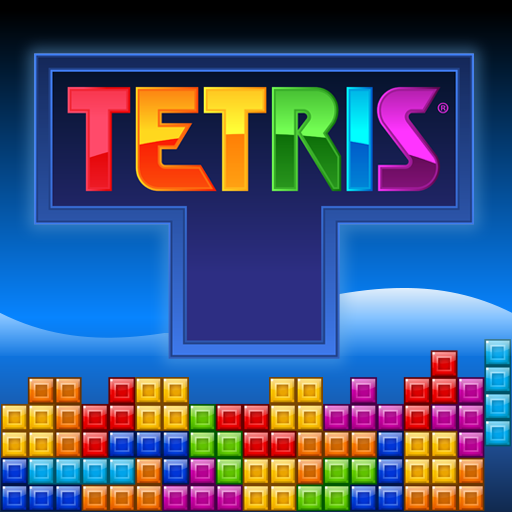
\includegraphics[scale=0.25]{10-tetris battle/tetris.png}
\end{center}

เกมก็เล่นง่ายๆ มีแค่ต่อบล็อกลงในกรอบขนาด $20 \times 10$ หน่วย ถ้าสามารถทำให้แถวไหนเต็มได้ แถวดังกล่าวก็จะหายไป (ไม่เกี่ยวกับคำถามในโจทย์)

ก็อย่างที่ได้รู้กันไปในโจทย์ช่วงเช้าแล้วว่าท่านธนพนธ์ ไม่เสื่อมสุข หรือ ToroTN เขาเป็นบุคคลที่เทพมากๆ นั่นรวมถึงการเล่นเกม Tetris ด้วย

ในวันหนึ่งท่าน ToroTN ได้เล่นเกม Tetris กับคนอื่นๆ ประกอบด้วย Jomnoiz (หรือ Jomnoi?), peteza และ ผู้เล่นอื่นๆ ได้แข่ง Tetris กันในช่วงดึก ซึ่งฝีมือของท่าน ToroTN สามารถตบทุกคนได้หมดในเกมส่วนใหญ่ 

แต่จากการเล่นมาหลายรอบจึงอาจทำให้ ToroTN สามารถพลาดได้บ้าง ซึ่งอาจจะโดน Jomnoiz หรือ peteza ตบในตานั้น ด้วยความโหดของ Jomnoiz ที่เป็นถึงระดับผู้แทนประเทศ เขาจึงได้รับคำชมจาก ToroTN (คิดโดย M-W?) ว่า

\begin{center}
    ผมก็บอกไปกี่ครั้งแล้ว ว่าต่อให้ใครต่อใครจะเก่งแค่ไหนอ่ะ ก็ไม่โหดเท่าคนที่ชื่อว่า \emph{\#จอม} \emph{\#จอมน้อย} \emph{\#จอมน้อยส์} \\
    \emph{\#Jomnoi} \emph{\#JomnoiZ} \emph{\#khem\_jomz} \emph{\#เขมอันเดอร์สกอร์จอมส์}  \emph{\#Kamanun Maneesri} \emph{\#เขมนันท์ มณีศรี} \\
    \emph{\#jomlovejen7956} \emph{\#จอมเลิฟเจนเจ็ดเก้าห้าหก} \emph{\#khem7956} \emph{\#เขมเจ็ดเก้าห้าหก}
\end{center}

เขายังโดนกวนสมาธิด้วยวิธิอื่น ๆ อย่างเช่นการ mentioned เนื่องจากหากโดน mentioned ในเกมนี้จะขึ้นเป็นตัวอักษร \textcolor{red}{สีแดง} \\(ตัวอย่างเช่นมีคำพิมพ์ว่า Jomnoiz เขาก็จะเห็นข้อความเป็น \textcolor{red}{Jomnoiz} ตามภาพ) ซึ่งอาจทำให้ผู้เล่นคนนั้นเสียสมาธิได้

\begin{center}
    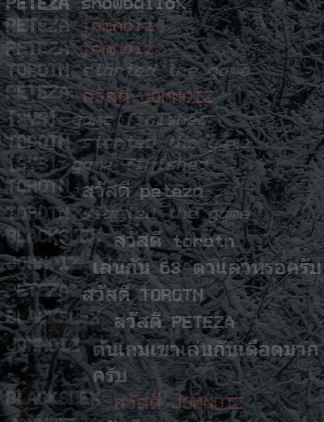
\includegraphics[scale=0.3]{10-tetris battle/tetris-chat.png}
\end{center}

นอกจากนี้ยังมีอีกผู้เล่นที่มีความสามารถในการเล่นเกมนี้เข้าขั้นแย่เลย นั่นก็คือ Blackslex จากที่เขาเล่นเกมนี้แย่ ทำให้โดนโจมตีจนตายอย่างรวดเร็ว เวลาว่างของเขาจึงมากจึงได้นำข้อความของ ToroTN ด้านบนมาแปลงเพื่อปั่น ToroTN อีกทีว่า

\begin{center}
    ผมก็บอกไปกี่ครั้งแล้วว่าต่อให้ใครจะเก่งแค่ไหนก็ไม่โหดเท่าคนที่ชื่อว่า \emph{\#ป้อน} \emph{\#pon} \emph{\#ponplayponplay} \emph{\#torotn} \emph{\#ponponzagggg}
\end{center}

หลังจากเขาได้ปั่น ToroTN มานานพอสมควร ทำให้เขาอยากเพิ่มระดับความเก่งของเขาบ้าง เขาได้ลุกขึ้นจากเก้าอี้เพื่อจะไปสถานที่บางแห่งแต่กลับเดินสะดุดสายไฟล้ม ข้ามผ่านประตูทะลุมิติไปยังอดีตในช่วงที่เคยมีผู้เล่น Tetris ที่เก่งที่สุดในโลกอยู่ ซึ่งผู้เล่นคนนี้ได้เก็บคัมภีร์เทคนิคลับไว้อยู่ในห้องใต้ดินลับสุดยอด ซึ่ง Blackslex ผู้เล่นที่เล่นได้แย่ที่สุดในคนที่แข่ง Tetris กันก็อยากได้เทคนิคลับนี้มาเอาชนะคนอื่นให้ได้ แต่นอกจาก Blackslex จะเล่น Tetris ได้แย่ที่สุดแล้ว ยังมีความสามารถในการประมวลผลข้อมูลต่ำมากอีกด้วย เขาจึงต้องการให้พวกคุณช่วยในการไขปริศนานี้ ซึ่งปัญหานี้มีอยู่ว่า \\
มี string $S$ ขนาด $N$ หลัก ซึ่งหลักแรกเริ่มนับเป็นหลักที่ $1$ แต่ละหลักประกอบด้วยเลขโดด $0$ ถึง $9$ โดยปัญหานั่นมีอยู่ $2$ รูปแบบ \\
รูปแบบที่ $1$ จะได้รับข้อมูล $a, b$ ซึ่งจะให้เปลี่ยนข้อมูลของ string $S$ ในหลักที่ $a$ ให้เป็น $b$ \\
ส่วนรูปแบบที่ $2$ จะได้รับข้อมูล $a, b$ เช่นกัน แต่จะให้ส่งกลับข้อมูลเป็นจำนวนเต็ม $1$ จำนวน แทนจำนวนของ substring ของ $S$ ในช่วง $a$ ถึง $b$ ที่หารด้วย $3$ ลงตัว หรือ อธิบายอีกอย่างนั่นก็คือ ให้หาจำนวนคู่ของ $x, y$ ที่ $S_xS_{x+1}\dots S_y$ เป็นหารด้วย $3$ ลงตัว และ เป็นส่วนหนึ่งของ string $S_aS_{a+1}\dots S_b$

\InputFile

บรรทัดแรก ระบุจำนวนเต็ม $N, Q$ $(1 \leq N, Q \leq 10^5)$

บรรทัดที่ $2$ มี จำนวนเต็ม $N$ จำนวน ระบุ $S_i$ แทนหลักที่ $i$ ของ $S$ $(1 \leq i \leq N, 0 \leq S_i \leq 9)$

บรรทัดที่ $3$ ถึง $Q + 2$ ระบุจำนวนเต็ม $M, a, b$ โดยที่ $M$ แทนประเภทคำถาม \\
ประเภทที่ $1$ $(M = 1)$ คือ เปลี่ยนค่า $S_a$ เป็น $b$ $(1 \leq a \leq N, 0 \leq b \leq 9)$ และ \\
ประเภทที่ $2$ $(M = 2)$ คือ หาจำนวน substring ของ $S_aS_{a+1}\dots S_b$ ที่หารด้วย $3$ ลงตัว $(1 \leq a \leq b \leq N)$

\OutputFile
มีไม่เกิน $Q$ บรรทัด ตามจำนวนคำถามที่ $M = 2$

\Scoring
ชุดทดสอบจะถูกแบ่งเป็น 4 ชุด จะได้คะแนนในแต่ละชุดก็ต่อเมื่อโปรแกรมให้ผลลัพธ์ถูกต้องในชุดทดสอบย่อยทั้งหมด

\begin{description}

\item[ชุดที่ 1 (12 คะแนน)] จะมี $ 1 \leq N, Q \leq 10^3$ และ $M = 2$
\item[ชุดที่ 2 (18 คะแนน)] จะมี $ 1 \leq N, Q \leq 10^3$
\item[ชุดที่ 3 (28 คะแนน)] จะมี $ 1 \leq N, Q \leq 10^5$ และ $M = 2$
\item[ชุดที่ 4 (42 คะแนน)] ไม่มีเงื่อนไขเพิ่มเติม 

\end{description}

\Examples

\begin{example}
\exmp{4 1
1234
2 1 2
}{1
}%
\exmp{4 2
1234
1 1 4
2 1 2
}{1
}%
\end{example}

\end{problem}

\end{document}
